\documentclass{ximera}
%\usepackage{todonotes}

\newcommand{\todo}{}

\usepackage{tkz-euclide}
\tikzset{>=stealth} %% cool arrow head
\tikzset{shorten <>/.style={ shorten >=#1, shorten <=#1 } } %% allows shorter vectors

\usepackage{tkz-tab}  %% sign charts
\usetikzlibrary{decorations.pathreplacing} 

\usetikzlibrary{backgrounds} %% for boxes around graphs
\usetikzlibrary{shapes,positioning}  %% Clouds and stars
\usetikzlibrary{matrix} %% for matrix
\usepgfplotslibrary{polar} %% for polar plots
\usetkzobj{all}
\usepackage[makeroom]{cancel} %% for strike outs
%\usepackage{mathtools} %% for pretty underbrace % Breaks Ximera
\usepackage{multicol}

\usepackage{polynom}



\usepackage[many]{tcolorbox}  %% for titled boxes
\newtcolorbox{xbox}[1]{%
    tikznode boxed title,
    enhanced,
    arc=0mm,
    interior style={white},
    attach boxed title to top center= {yshift=-\tcboxedtitleheight/2},
    fonttitle=\bfseries,
    colbacktitle=white,coltitle=black,
    boxed title style={size=normal,colframe=white,boxrule=0pt},
    title={#1}}


\usepackage{array}
\setlength{\extrarowheight}{+.1cm}   
\newdimen\digitwidth
\settowidth\digitwidth{9}
\def\divrule#1#2{
\noalign{\moveright#1\digitwidth
\vbox{\hrule width#2\digitwidth}}}





\newcommand{\RR}{\mathbb R}
\newcommand{\R}{\mathbb R}
\newcommand{\N}{\mathbb N}
\newcommand{\Z}{\mathbb Z}

%\renewcommand{\d}{\,d\!}
\renewcommand{\d}{\mathop{}\!d}
\newcommand{\dd}[2][]{\frac{\d #1}{\d #2}}
\newcommand{\pp}[2][]{\frac{\partial #1}{\partial #2}}
\renewcommand{\l}{\ell}
\newcommand{\ddx}{\frac{d}{\d x}}
\newcommand{\ddt}{\frac{d}{\d t}}

\newcommand{\zeroOverZero}{\ensuremath{\boldsymbol{\tfrac{0}{0}}}}
\newcommand{\inftyOverInfty}{\ensuremath{\boldsymbol{\tfrac{\infty}{\infty}}}}
\newcommand{\zeroOverInfty}{\ensuremath{\boldsymbol{\tfrac{0}{\infty}}}}
\newcommand{\zeroTimesInfty}{\ensuremath{\small\boldsymbol{0\cdot \infty}}}
\newcommand{\inftyMinusInfty}{\ensuremath{\small\boldsymbol{\infty - \infty}}}
\newcommand{\oneToInfty}{\ensuremath{\boldsymbol{1^\infty}}}
\newcommand{\zeroToZero}{\ensuremath{\boldsymbol{0^0}}}
\newcommand{\inftyToZero}{\ensuremath{\boldsymbol{\infty^0}}}



\newcommand{\numOverZero}{\ensuremath{\boldsymbol{\tfrac{\#}{0}}}}
\newcommand{\dfn}{\textbf}
%\newcommand{\unit}{\,\mathrm}
\newcommand{\unit}{\mathop{}\!\mathrm}
\newcommand{\eval}[1]{\bigg[ #1 \bigg]}
\newcommand{\seq}[1]{\left( #1 \right)}
\renewcommand{\epsilon}{\varepsilon}
\renewcommand{\iff}{\Leftrightarrow}

\DeclareMathOperator{\arccot}{arccot}
\DeclareMathOperator{\arcsec}{arcsec}
\DeclareMathOperator{\arccsc}{arccsc}
\DeclareMathOperator{\si}{Si}
\DeclareMathOperator{\proj}{proj}
\DeclareMathOperator{\scal}{scal}


\newcommand{\tightoverset}[2]{% for arrow vec
  \mathop{#2}\limits^{\vbox to -.5ex{\kern-0.75ex\hbox{$#1$}\vss}}}
\newcommand{\arrowvec}[1]{\tightoverset{\scriptstyle\rightharpoonup}{#1}}
\renewcommand{\vec}{\mathbf}
\newcommand{\veci}{\vec{i}}
\newcommand{\vecj}{\vec{j}}
\newcommand{\veck}{\vec{k}}
\newcommand{\vecl}{\boldsymbol{\l}}

\newcommand{\dotp}{\bullet}
\newcommand{\cross}{\boldsymbol\times}
\newcommand{\grad}{\boldsymbol\nabla}
\newcommand{\divergence}{\grad\dotp}
\newcommand{\curl}{\grad\cross}
%\DeclareMathOperator{\divergence}{divergence}
%\DeclareMathOperator{\curl}[1]{\grad\cross #1}


\colorlet{textColor}{black} 
\colorlet{background}{white}
\colorlet{penColor}{blue!50!black} % Color of a curve in a plot
\colorlet{penColor2}{red!50!black}% Color of a curve in a plot
\colorlet{penColor3}{red!50!blue} % Color of a curve in a plot
\colorlet{penColor4}{green!50!black} % Color of a curve in a plot
\colorlet{penColor5}{orange!80!black} % Color of a curve in a plot
\colorlet{fill1}{penColor!20} % Color of fill in a plot
\colorlet{fill2}{penColor2!20} % Color of fill in a plot
\colorlet{fillp}{fill1} % Color of positive area
\colorlet{filln}{penColor2!20} % Color of negative area
\colorlet{fill3}{penColor3!20} % Fill
\colorlet{fill4}{penColor4!20} % Fill
\colorlet{fill5}{penColor5!20} % Fill
\colorlet{gridColor}{gray!50} % Color of grid in a plot

\newcommand{\surfaceColor}{violet}
\newcommand{\surfaceColorTwo}{redyellow}
\newcommand{\sliceColor}{greenyellow}




\pgfmathdeclarefunction{gauss}{2}{% gives gaussian
  \pgfmathparse{1/(#2*sqrt(2*pi))*exp(-((x-#1)^2)/(2*#2^2))}%
}


%%%%%%%%%%%%%
%% Vectors
%%%%%%%%%%%%%

%% Simple horiz vectors
\renewcommand{\vector}[1]{\left\langle #1\right\rangle}


%% %% Complex Horiz Vectors with angle brackets
%% \makeatletter
%% \renewcommand{\vector}[2][ , ]{\left\langle%
%%   \def\nextitem{\def\nextitem{#1}}%
%%   \@for \el:=#2\do{\nextitem\el}\right\rangle%
%% }
%% \makeatother

%% %% Vertical Vectors
%% \def\vector#1{\begin{bmatrix}\vecListA#1,,\end{bmatrix}}
%% \def\vecListA#1,{\if,#1,\else #1\cr \expandafter \vecListA \fi}

%%%%%%%%%%%%%
%% End of vectors
%%%%%%%%%%%%%

%\newcommand{\fullwidth}{}
%\newcommand{\normalwidth}{}



%% makes a snazzy t-chart for evaluating functions
%\newenvironment{tchart}{\rowcolors{2}{}{background!90!textColor}\array}{\endarray}

%%This is to help with formatting on future title pages.
\newenvironment{sectionOutcomes}{}{} 



%% Flowchart stuff
%\tikzstyle{startstop} = [rectangle, rounded corners, minimum width=3cm, minimum height=1cm,text centered, draw=black]
%\tikzstyle{question} = [rectangle, minimum width=3cm, minimum height=1cm, text centered, draw=black]
%\tikzstyle{decision} = [trapezium, trapezium left angle=70, trapezium right angle=110, minimum width=3cm, minimum height=1cm, text centered, draw=black]
%\tikzstyle{question} = [rectangle, rounded corners, minimum width=3cm, minimum height=1cm,text centered, draw=black]
%\tikzstyle{process} = [rectangle, minimum width=3cm, minimum height=1cm, text centered, draw=black]
%\tikzstyle{decision} = [trapezium, trapezium left angle=70, trapezium right angle=110, minimum width=3cm, minimum height=1cm, text centered, draw=black]

\author{Steven Gubkin\and Nela Lakos}
\license{Creative Commons 3.0 By-NC}

\outcome{Define linear approximation as an application of the tangent to a curve.}
\outcome{Find the linear approximation to a function at a point and use it to approximate the function value.}
\outcome{Identify when a linear approximation can be used.}
\begin{document}
\begin{exercise}

Approximate $\sqrt{9.5}$ by hand using the idea of linear approximation (of a conveniently chosen function, and base point).  Using the second derivative, explain whether you think this is an underestimate or an overestimate.
\begin {hint}

The number that you have to approximate should be expressed as

 $\sqrt{9.5}=f(x)$.
Obviously, $f(x)=\sqrt{x}$, and $x=9.5$.
\end {hint}
\begin {hint}

You will now approximate  $\sqrt{9.5}=f(x)$
 with $L (x)$, where $L$ is the linear approximation of $f$ at $a$.
In other words, $\sqrt{9.5}=f(x)\approx L(x)$.

 You have to choose the "base" number $a$  wisely, so that $x=9.5$ is near $a$, and so that you can easily and exactly compute the values $f(a)$ and $f'(a)$.
 These two values are needed when we compute the expression for $L(x)$. 
\end {hint}
\begin {hint}
The obvious choice for $a$ is $a=9$. Any other number for which it is easy to compute $\sqrt{a}$ is farther away from $x=9.5$.
Now we have to compute $f(a)=f(9)$ and $f'(a)=f'(9)$.
\begin{prompt}
	$$f(9)=  \answer{3}$$
	\end{prompt}
	\begin{prompt}
	$$f'(x)= \frac{1}{ \answer{2\sqrt{x}}}$$
	\end{prompt}
	\begin{prompt}
	$$f'(9)= \frac{1}{ \answer{6}}$$
	\end{prompt}
\end {hint}
\begin {hint}

Now, we have to find an expression for $L(x)=f(9)+f'(9)(x-9)$.
\begin{prompt}
	$$L(x)= \answer{3}+\answer{\frac{1}{6}}(x-9)$$
	\end{prompt}
 
\end {hint}
\begin {hint}

Now, we have to evaluate $L(x)=L(9.5)$.
\begin{prompt}
	$$L(9.5)= \answer{3}+\answer{\frac{1}{6}}(9.5-9)$$
	\end{prompt}
 
\end {hint}
\begin{prompt}
	$$\sqrt{9.5} \approx \answer{3+\frac{1}{12}}$$
Is this an underestimate or overestimate?
\begin{hint}
 \begin{image}
%\begin{marginfigure}
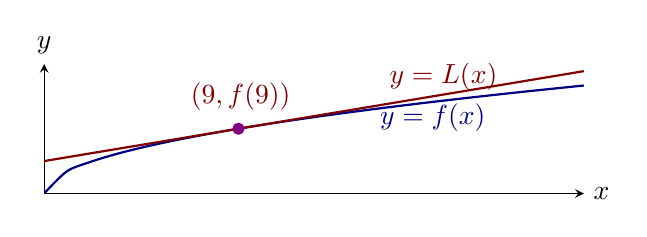
\begin{tikzpicture}
	\begin{axis}[
            xmin=0,xmax=25,ymin=0,ymax=6,
            axis lines=center,
            ticks=none,
            %width=3in,
            %height=2in,
            unit vector ratio*=1 1 1,
            xlabel=$x$, ylabel=$y$,
            every axis y label/.style={at=(current axis.above origin),anchor=south},
            every axis x label/.style={at=(current axis.right of origin),anchor=west},
          ]        
          \addplot [ thick, penColor, smooth, domain=(0:25)] {sqrt(x)};
          \addplot [thick, penColor2,smooth, domain=(0:25)] {3+(1/6)*(x-9)};
          \node at (axis cs:18,3.5) [penColor] {$y=f(x)$};
          \node at (axis cs:18.5,5.4) [penColor2] {$y=L(x)$}; 
          \node at (axis cs:9.1,4.5) [penColor2] {$(9,f(9))$}; 
            \addplot[color=penColor3,fill=penColor3,only marks,mark=*] coordinates{(9,3)};  %% closed hole         
        \end{axis}
\end{tikzpicture}
%\caption{A linear approximation of $f(x) = \sin(x)$ at $x=0$.}
%\label{figure:la sin}
%\end{marginfigure}
\end{image}
\end{hint}
\begin {hint}
Recall: $f''(x)=-\frac{1}{4\cdot x^{\answer{\frac{3}{2}}}}$. 

Since $f''(x)<0$ on $(0,\infty)$,  the graph of $f$ is concave down. Therefore, the tangent line lies above the graph of $f$, except at $x=9$, where $f(9)=L(9)$.


This means that $L(x)\ge f(x)$. So, $L(9.5)\ge f(9.5)$.
\end{hint}
This is an
\begin{multipleChoice}
   \choice{underestimate}
   \choice[correct]{overestimate}
\end{multipleChoice}
\end{prompt}

\end{exercise}
\end{document}
